\documentclass[11pt,a4paper]{article}

% ---------------------------------------------------------------- packages
\usepackage[T1]{fontenc}
\usepackage{lmodern}
\usepackage{microtype}
\usepackage[margin=2.3cm,headheight=14pt]{geometry}
\usepackage[dvipsnames,table]{xcolor}
\usepackage{amsmath,amssymb}
\usepackage{booktabs,tabularx,array,longtable,makecell}
\usepackage{enumitem}
\usepackage{listings}
\usepackage{tikz}
\usetikzlibrary{positioning,arrows.meta,fit,backgrounds,shapes.geometric,calc}
\usepackage[most]{tcolorbox}
\usepackage{fancyhdr}
\usepackage{titlesec}
\usepackage{needspace}
\usepackage[hidelinks]{hyperref}

% ---------------------------------------------------------------- colours
\definecolor{ink}{HTML}{1F2937}
\definecolor{accent}{HTML}{1D4ED8}
\definecolor{accentlight}{HTML}{DBEAFE}
\definecolor{good}{HTML}{047857}
\definecolor{goodlight}{HTML}{D1FAE5}
\definecolor{warn}{HTML}{B45309}
\definecolor{warnlight}{HTML}{FEF3C7}
\definecolor{bad}{HTML}{B91C1C}
\definecolor{badlight}{HTML}{FEE2E2}
\definecolor{grey}{HTML}{6B7280}
\definecolor{greylight}{HTML}{F3F4F6}
\definecolor{purple1}{HTML}{6D28D9}
\definecolor{purplelight}{HTML}{EDE9FE}

\color{ink}

% ---------------------------------------------------------------- layout
\setlength{\parindent}{0pt}
\setlength{\emergencystretch}{3em}
\setlength{\parskip}{6pt}
\setlist{itemsep=2pt,topsep=3pt}
\renewcommand{\arraystretch}{1.25}

\titleformat{\section}{\needspace{12\baselineskip}\Large\bfseries\color{accent}}{\thesection}{0.8em}{}
\titleformat{\subsection}{\needspace{7\baselineskip}\large\bfseries\color{ink}}{\thesubsection}{0.7em}{}
\titleformat{\subsubsection}{\normalsize\bfseries\color{ink}}{\thesubsubsection}{0.6em}{}
\titlespacing*{\section}{0pt}{18pt}{8pt}
\titlespacing*{\subsection}{0pt}{12pt}{5pt}

\pagestyle{fancy}
\fancyhf{}
\fancyhead[L]{\small\color{grey}QueryLens: Project Charter and Data Specification}
\fancyhead[R]{\small\color{grey}\nouppercase{\leftmark}}
\fancyfoot[C]{\small\color{grey}\thepage}
\renewcommand{\headrulewidth}{0.4pt}

% ---------------------------------------------------------------- boxes
\newtcolorbox{keybox}[1]{enhanced,breakable,colback=accentlight,colframe=accent,
  boxrule=0.6pt,arc=2pt,left=8pt,right=8pt,top=6pt,bottom=6pt,
  fonttitle=\bfseries,title={#1}}
\newtcolorbox{goodbox}[1]{enhanced,breakable,colback=goodlight,colframe=good,
  boxrule=0.6pt,arc=2pt,left=8pt,right=8pt,top=6pt,bottom=6pt,
  fonttitle=\bfseries,title={#1}}
\newtcolorbox{warnbox}[1]{enhanced,breakable,colback=warnlight,colframe=warn,
  boxrule=0.6pt,arc=2pt,left=8pt,right=8pt,top=6pt,bottom=6pt,
  fonttitle=\bfseries,title={#1}}
\newtcolorbox{plainbox}{enhanced,breakable,colback=greylight,colframe=greylight,
  boxrule=0pt,arc=2pt,left=8pt,right=8pt,top=6pt,bottom=6pt}

% ---------------------------------------------------------------- code
\lstdefinestyle{code}{
  basicstyle=\ttfamily\footnotesize,
  keywordstyle=\color{accent}\bfseries,
  commentstyle=\color{grey}\itshape,
  stringstyle=\color{good},
  backgroundcolor=\color{greylight},
  frame=single, rulecolor=\color{greylight},
  framexleftmargin=4pt, xleftmargin=4pt,
  breaklines=true, columns=fullflexible, keepspaces=true,
  showstringspaces=false, upquote=true, tabsize=4,
  aboveskip=6pt, belowskip=6pt
}
\lstset{style=code}
\lstdefinelanguage{yaml}{keywords={true,false,null},sensitive=false,
  comment=[l]{\#}, morestring=[b]", morestring=[b]'}

% ---------------------------------------------------------------- tikz styles
\tikzset{
  box/.style={draw=accent,fill=accentlight,rounded corners=3pt,thick,
              align=center,font=\small,minimum height=1.0cm,inner sep=4pt},
  gbox/.style={box,draw=good,fill=goodlight},
  wbox/.style={box,draw=warn,fill=warnlight},
  rbox/.style={box,draw=bad,fill=badlight},
  pbox/.style={box,draw=purple1,fill=purplelight},
  nbox/.style={box,draw=grey,fill=greylight},
  arr/.style={-{Stealth[length=2.6mm]},thick,draw=ink},
  darr/.style={arr,dashed},
  lbl/.style={font=\scriptsize\itshape,text=grey,align=center},
  group/.style={draw=grey,dashed,rounded corners=5pt,inner sep=8pt},
  grouplbl/.style={font=\footnotesize\bfseries,text=grey}
}

\newcommand{\code}[1]{\texttt{\small #1}}
\newcommand{\tick}{\textcolor{good}{\checkmark}}

% =====================================================================
\begin{document}

% ---------------------------------------------------------------- title
\begin{titlepage}
\thispagestyle{empty}
\vspace*{1.5cm}
{\color{grey}\large PROJECT CHARTER AND DATA SPECIFICATION}\\[6pt]
{\color{accent}\rule{\linewidth}{1.2pt}}\\[14pt]
{\fontsize{30}{36}\selectfont\bfseries QueryLens}\\[10pt]
{\Large Evaluation-Driven Development of a Text-to-SQL Analyst Agent on a Multi-Domain
E-commerce Data Warehouse}\\[10pt]
{\color{accent}\rule{\linewidth}{1.2pt}}

\vspace{1cm}
\begin{center}
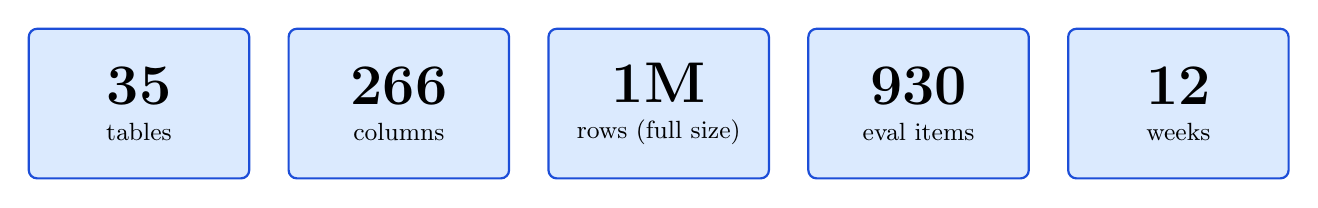
\begin{tikzpicture}
  \foreach \x/\n/\l in {0/35/tables, 3.3/266/columns, 6.6/1M/rows (full size), 9.9/930/eval items, 13.2/12/weeks}{
    \node[box,minimum width=2.8cm,minimum height=1.9cm,align=center] at (\x,0)
      {{\fontsize{20}{24}\selectfont\bfseries \n}\\[2pt]\small \l};
  }
\end{tikzpicture}
\end{center}

\vfill
\begin{tabularx}{\linewidth}{@{}lX@{}}
\textbf{Document} & Project charter and data specification, version 1.0\\
\textbf{Companions} & \emph{QueryLens Design Document v2} (architecture and method); \code{CLAUDE.md} (implementation brief for Claude Code)\\
\textbf{Owner} & [your name]\\
\textbf{Date} & November 2026\\
\end{tabularx}
\end{titlepage}

\tableofcontents
\newpage

% =====================================================================
\section{Project Identity}

\begin{center}
\begin{tabularx}{\linewidth}{@{}>{\bfseries}l X@{}}
\toprule
Full name & QueryLens: Evaluation-Driven Development of a Text-to-SQL Analyst Agent on a Multi-Domain E-commerce Data Warehouse\\
Short name & QueryLens\\
Tagline & ``Ask the warehouse in plain words, and know when to trust the answer.''\\
Database name & BazaarDW (Bazaar Data Warehouse), a synthetic warehouse for a fictional Bangladeshi online marketplace called \emph{Bazaar}\\
Library name & \code{evalkit} (evaluation toolkit, reusable for other LLM products)\\
Repository & \code{querylens} (one repository, MIT licence)\\
Python packages & \code{querylens} (agent), \code{evalkit} (evals), \code{bazaar\_world} (data generator)\\
Project type & Portfolio project: AI engineering and LLM evaluation\\
LLM access & Free tiers only: Mistral, Google Gemini, Groq, OpenRouter \code{:free}, plus local Ollama (\$0 API spend)\\
Source material & \emph{AI Evals For Engineers \& PMs} syllabus (L1--L9); \emph{AI Engineering Project Blueprint}, Project 5\\
\bottomrule
\end{tabularx}
\end{center}

\subsection{Summary}

QueryLens is an AI analyst that answers business questions about a large e-commerce warehouse
by finding the right tables, writing SQL, running it safely and explaining the result. The main
deliverable is not the agent but the \textbf{evaluation system} around it: a synthetic warehouse
with known facts, 930 evaluation items, a failure taxonomy built from reading real traces,
validated LLM judges, a CI gate that blocks regressions, a red-team suite, and a measured
accuracy--cost--latency frontier.

\subsection{Objectives}

\begin{center}
\small
\begin{tabularx}{\linewidth}{@{}l X l@{}}
\toprule
\textbf{ID} & \textbf{Objective} & \textbf{Measured by}\\
\midrule
O1 & Build a realistic, deterministic warehouse in two sizes (1 lakh and 10 lakh rows) & table hashes, row counts, planted-fact tests\\
O2 & Build an analyst agent that is safe by construction & guard tests; unsafe accesses = 0\\
O3 & Measure the agent with trustworthy evals & judges' TPR/TNR on frozen test labels\\
O4 & Catch regressions automatically & CI gate blocks a planted regression\\
O5 & Improve accuracy with evidence & paired comparison on the frozen test slice\\
O6 & Reduce tokens and latency without losing accuracy, on free tiers only & tokens per question, p95 latency, accuracy CI\\
\bottomrule
\end{tabularx}
\end{center}

\subsection{In scope and out of scope}

\begin{center}
\small
\begin{tabularx}{\linewidth}{@{}X X@{}}
\toprule
\textbf{In scope} & \textbf{Out of scope}\\
\midrule
One warehouse: 35 tables, 11 domains, 2 sizes & Real customer data of any kind\\
Read-only analytical questions in English & Any write operation on the database\\
Bangla and Banglish slices (stretch) & Distributed or cloud data warehouses\\
4 roles with code-enforced permissions & A production BI front end\\
7 agent tools, 24 semantic-layer metrics & Fine-tuning a model (unless the improvement phase justifies it)\\
Free-tier LLM APIs and local models & Any paid LLM API\\
Full evaluation, CI, red-teaming, optimisation & Public leaderboard submissions\\
\bottomrule
\end{tabularx}
\end{center}

% =====================================================================
\section{Deliverables}

\begin{center}
\small
\begin{tabularx}{\linewidth}{@{}l X l l@{}}
\toprule
\textbf{ID} & \textbf{Deliverable} & \textbf{Location} & \textbf{Week}\\
\midrule
D1 & \code{SPEC.md}: roles, tools, risk tiers, escalation & repo root & 1\\
D2 & BazaarDW generator, small and full sizes, seed 42 & \code{world/} & 1--2\\
D3 & Data dictionary (35 tables, 266 columns) and role views & \code{world/} & 2\\
D4 & Semantic layer: 24 metrics with reference SQL & \code{semantic/metrics.yaml} & 2\\
D5 & Analyst agent with 7 tools, guard and schema retriever & \code{src/querylens/} & 3\\
D6 & Tracer and trace store & \code{evalkit/trace.py} & 3\\
D7 & Eval datasets: 930 items with gold SQL and gold results & \code{datasets/} & 4\\
D8 & Trace viewer with annotation & \code{app/viewer.py} & 5\\
D9 & Error-analysis report and failure taxonomy & \code{docs/error\_analysis.md} & 5\\
D10 & Code evaluators, component evals, 3 validated judges & \code{evalkit/}, \code{rubrics/} & 6--7\\
D11 & CI workflows: PR gate and nightly suite & \code{.github/workflows/} & 8\\
D12 & Red-team suite and governance record & \code{redteam/}, \code{docs/governance.md} & 9\\
D13 & Frontier configs and optimisation report & \code{configs/}, \code{docs/report.md} & 10--11\\
D14 & README, frontier plot, demo GIF, public write-up & repo root & 12\\
\bottomrule
\end{tabularx}
\end{center}

% =====================================================================
\section{BazaarDW Data Specification}

\subsection{Global parameters}

\begin{center}
\small
\begin{tabularx}{\linewidth}{@{}l X@{}}
\toprule
\textbf{Parameter} & \textbf{Value}\\
\midrule
Random seed & 42 (every table is derived from the seed and the size only)\\
Time period & 2024-01-01 to 2026-10-31 (34 months, 1{,}035 days)\\
Geography & Bangladesh: 8 divisions (\code{regions}), 64 districts (\code{cities})\\
Base currency & BDT; 1.2\% of orders in USD, converted with \code{currency\_rates} on the order date\\
Time zones & Event timestamps in UTC (columns ending \code{\_utc}); business dates in Asia/Dhaka (UTC+6)\\
Weekend & Friday and Saturday (\code{calendar\_dim.is\_weekend})\\
Fiscal year & July to June (\code{calendar\_dim.fiscal\_year})\\
Engine & one DuckDB file per size; Parquet export per table\\
File names & \code{data/bazaar\_small.duckdb}, \code{data/bazaar\_full.duckdb}\\
\bottomrule
\end{tabularx}
\end{center}

\subsection{Sizes}

\begin{center}
\begin{tabular}{@{}l r r l@{}}
\toprule
\textbf{Size} & \textbf{Total rows} & \textbf{Approx.\ size} & \textbf{Purpose}\\
\midrule
small & 102{,}266 (1 lakh) & 5--10\,MB & unit tests, CI, quick experiments\\
full & 995{,}786 (10 lakh) & 40--80\,MB & PR checks, nightly, test slice, results\\
\bottomrule
\end{tabular}

{\footnotesize\color{grey} Nine small tables do not change between sizes: regions, cities, calendar\_dim,
currency\_rates, categories, couriers, warehouses, marketing\_campaigns, promotions. Every other table
in the small size has 10\% of the full rows. Sizes are estimates; record the measured sizes in the README.}
\end{center}

\subsection{Table catalogue}

{\footnotesize
\begin{longtable}{@{}l l r r r r >{\raggedright\arraybackslash}p{3.1cm}@{}}
\toprule
\textbf{Domain} & \textbf{Table} & \textbf{Small} & \textbf{Full} & \textbf{Cols} & \textbf{Size (full)} & \textbf{Notes}\\
\midrule
\endfirsthead
\toprule
\textbf{Domain} & \textbf{Table} & \textbf{Small} & \textbf{Full} & \textbf{Cols} & \textbf{Size (full)} & \textbf{Notes}\\
\midrule
\endhead
Reference & \code{regions} & 8 & 8 & 4 & $<$0.1 MB & 8 divisions\\
 & \code{cities} & 64 & 64 & 6 & $<$0.1 MB & 64 districts\\
 & \code{calendar\_dim} & 1,035 & 1,035 & 12 & $<$0.1 MB & 2024-01-01..2026-10-31\\
 & \code{currency\_rates} & 1,035 & 1,035 & 4 & $<$0.1 MB & daily BDT/USD\\
Customers & \code{customers} & 1,000 & 10,000 & 14 & 1.1 MB & PII: name, email, phone\\
 & \code{customer\_addresses} & 1,300 & 13,000 & 9 & 0.9 MB & PII: street\\
 & \code{customer\_segment\_history} & 1,600 & 16,000 & 6 & 0.7 MB & SCD type 2\\
 & \code{loyalty\_accounts} & 450 & 4,500 & 6 & 0.2 MB & \\
 & \code{loyalty\_transactions} & 3,600 & 36,000 & 7 & 1.9 MB & \\
Catalog & \code{categories} & 300 & 300 & 5 & $<$0.1 MB & 3-level tree\\
 & \code{brands} & 40 & 400 & 4 & $<$0.1 MB & \\
 & \code{products} & 400 & 4,000 & 12 & 0.4 MB & duplicate names on purpose\\
 & \code{product\_variants} & 1,100 & 11,000 & 8 & 0.7 MB & size/colour\\
 & \code{product\_price\_history} & 3,000 & 30,000 & 6 & 1.4 MB & SCD type 2\\
Sellers & \code{sellers} & 30 & 300 & 10 & $<$0.1 MB & \\
 & \code{seller\_tier\_history} & 70 & 700 & 5 & $<$0.1 MB & SCD type 2\\
 & \code{seller\_payouts} & 900 & 9,000 & 7 & 0.5 MB & \\
Inventory & \code{warehouses} & 12 & 12 & 6 & $<$0.1 MB & \\
 & \code{inventory\_snapshots} & 4,000 & 40,000 & 6 & 1.8 MB & weekly, variant $\times$ warehouse\\
Orders & \code{orders} & 5,500 & 55,000 & 13 & 5.4 MB & soft deletes, mixed status spellings\\
 & \code{order\_items} & 14,000 & 140,000 & 9 & 9.6 MB & \\
 & \code{order\_status\_events} & 17,000 & 170,000 & 5 & 6.5 MB & largest table; UTC timestamps\\
Payments & \code{payments} & 5,800 & 58,000 & 9 & 4.0 MB & retries create duplicates\\
 & \code{refunds} & 330 & 3,300 & 7 & 0.2 MB & \\
 & \code{returns} & 260 & 2,600 & 8 & 0.2 MB & \\
Logistics & \code{couriers} & 12 & 12 & 4 & $<$0.1 MB & \\
 & \code{shipments} & 5,600 & 56,000 & 10 & 4.3 MB & promised vs delivered dates\\
 & \code{shipment\_events} & 15,000 & 150,000 & 6 & 6.8 MB & \\
Marketing & \code{marketing\_campaigns} & 120 & 120 & 8 & $<$0.1 MB & \\
 & \code{promotions} & 400 & 400 & 9 & $<$0.1 MB & \\
 & \code{promotion\_redemptions} & 1,500 & 15,000 & 6 & 0.7 MB & \\
Web & \code{web\_sessions} & 12,000 & 120,000 & 11 & 10.0 MB & \\
Support & \code{support\_tickets} & 500 & 5,000 & 10 & 0.4 MB & \\
 & \code{support\_messages} & 2,500 & 25,000 & 6 & 1.1 MB & untrusted free text\\
Reviews & \code{product\_reviews} & 1,800 & 18,000 & 8 & 1.1 MB & untrusted free text\\
\midrule
\textbf{Total} & \textbf{35 tables} & \textbf{102,266} & \textbf{995,786} & \textbf{266} & \textbf{$\approx$60 MB} & \\
\bottomrule
\end{longtable}
}
{\footnotesize\color{grey} Size per table is an estimate proportional to rows $\times$ columns.}

\subsection{Generator distributions}

These parameters make the data behave like a real marketplace, so that analytical questions
have interesting answers. They are inputs to the generator, defined in \code{world/params.yaml}.

\begin{center}
\small
\begin{tabularx}{\linewidth}{@{}l X@{}}
\toprule
\textbf{Aspect} & \textbf{Generator setting}\\
\midrule
Customer activity & Pareto: top 20\% of customers place about 65\% of orders; 35\% of customers order once only\\
Order channel & app 62\%, web 30\%, social commerce 8\%\\
Payment method & bKash 38\%, cash on delivery 30\%, Nagad 14\%, card 12\%, bank transfer 6\%\\
Payment retries & 9\% of orders have at least one failed attempt before capture\\
Order status & delivered 82\%, cancelled 7\% (60\% spelled 'cancelled', 40\% 'canceled'), in transit 5\%, returned 3\%, payment failed 3\%\\
Seasonality & weekly cycle; Eid al-Fitr and Eid al-Adha weeks $\times$2.4 and $\times$1.8; 11.11 sale $\times$3.0; Pohela Boishakh $\times$1.5\\
Growth & orders grow about 3\% per month over the period\\
Refunds & baseline refund rate 4.5\%; planted spike of 9.4\% in Chattogram, March 2026\\
Deliveries & baseline late-delivery rate 12\%, varying by courier (6--21\%) and division\\
Reviews & ratings 5: 48\%, 4: 24\%, 3: 11\%, 2: 6\%, 1: 11\%; 32\% of delivered orders get a review\\
Soft deletes & 0.4\% of orders and 1\% of products have \code{is\_deleted = true}\\
Duplicate names & 1.5\% of product names are shared by two or more products\\
History tables & 18\% of sellers change tier at least once; prices change on average every 70 days\\
Injected text & 40 reviews and 25 support messages contain prompt-injection text (fixed rows, both sizes)\\
\bottomrule
\end{tabularx}
\end{center}

\subsection{Personal data and role access}

Columns marked \textcolor{bad}{red} in the appendix are personal data (PII). Columns marked
\textcolor{warn}{orange} are untrusted free text. Access is granted through role schemas of views.

\begin{center}
\small
\begin{tabular}{@{}l c c c c@{}}
\toprule
\textbf{Data} & \code{analyst} & \code{support\_lead} & \code{finance} & \code{admin}\\
\midrule
Business tables (orders, items, products, shipments, \ldots) & \tick & \tick & partial & \tick\\
Customer name & & \tick & & \tick\\
Customer email, phone, street address, postcode & & & & \tick\\
Seller contact email and phone & & & & \tick\\
Support message text & & \tick & & \tick\\
Payments, refunds, payouts & \tick & \tick & \tick & \tick\\
\bottomrule
\end{tabular}
\end{center}

\subsection{Semantic layer: the 24 metrics}

\begin{center}
\small
\begin{tabularx}{\linewidth}{@{}l X l X@{}}
\toprule
\textbf{Metric} & \textbf{Definition} & \textbf{Metric} & \textbf{Definition}\\
\midrule
\code{gmv} & Sum of order line totals before refunds & \code{net\_revenue} & Captured payments minus refunds\\
\code{order\_count} & Non-deleted, non-cancelled orders & \code{aov} & net\_revenue / order\_count\\
\code{items\_per\_order} & Mean item quantity per order & \code{active\_customers} & Customers with $\geq$1 order in period\\
\code{new\_customers} & First order falls in period & \code{repeat\_rate} & Share of customers with $\geq$2 orders\\
\code{cancellation\_rate} & Cancelled / all orders (both spellings) & \code{refund\_rate} & Orders with a refund / orders\\
\code{return\_rate} & Returned items / delivered items & \code{payment\_success} & Captured / all payment attempts\\
\code{cod\_share} & Cash-on-delivery orders / orders & \code{late\_delivery\_rate} & Delivered late / delivered (Dhaka dates)\\
\code{avg\_delivery\_days} & Mean days, shipped to delivered & \code{active\_sellers} & Sellers with $\geq$1 sale in period\\
\code{seller\_payout} & Gross minus commission, paid & \code{promo\_redemption\_rate} & Orders with a promo / orders\\
\code{discount\_cost} & Sum of discounts given & \code{session\_conversion} & Sessions with an order / sessions\\
\code{avg\_rating} & Mean review rating & \code{ticket\_resolution\_h} & Median hours to resolve a ticket\\
\code{stockout\_rate} & Snapshots with on-hand = 0 / snapshots & \code{points\_redeemed} & Loyalty points spent\\
\bottomrule
\end{tabularx}
\end{center}

\subsection{Planted facts}

The generator writes these facts on purpose, in both sizes, and records
them in \code{world/facts.yaml}. They give questions with known answers.

\begin{center}
\small
\begin{tabularx}{\linewidth}{@{}l X l@{}}
\toprule
\textbf{ID} & \textbf{Fact} & \textbf{Tests}\\
\midrule
F01 & Seller ``Padma Gadgets'' has the highest late-delivery rate in 2026-Q3 among sellers with 300+ shipments (30+ in the small size) & ranking\\
F02 & Refund rate spikes to 9.4\% in Chattogram in March 2026 (courier FastBox) & ratio, geography\\
F03 & Two different products are named ``Classic Panjabi'' & ambiguity\\
F04 & Seller ``Meghna Mart'' moves from silver to gold tier on 2025-07-01 & SCD2 join\\
F05 & 11.11 sale day 2025 is the highest-GMV day in the period & trend, calendar\\
F06 & Customers acquired by the ``Boishakh25'' campaign have the best 90-day repeat rate & cohort\\
F07 & bKash payment success drops to 81\% for 3 days in August 2025 (outage) & time series\\
F08 & Warehouse ``Gazipur-2'' has the highest stockout rate in 2026 & inventory\\
\bottomrule
\end{tabularx}
\end{center}

% =====================================================================
\section{Evaluation Data Specification}

\subsection{Item counts by set and split}

\begin{center}
\begin{tabular}{@{}l r r r r@{}}
\toprule
\textbf{Set} & \textbf{Train} & \textbf{Dev} & \textbf{Test} & \textbf{Total}\\
\midrule
Golden (answerable, gold SQL) & 120 & 120 & 160 & 400\\
Ambiguous (expect clarification) & 24 & 24 & 32 & 80\\
Unanswerable (expect abstention) & 18 & 18 & 24 & 60\\
Adversarial (expect refusal or safe handling) & --- & 60 & 90 & 150\\
Bilingual: English + Bangla (60 pairs) & --- & 60 & 60 & 120\\
Bilingual: English + Banglish (60 pairs) & --- & 60 & 60 & 120\\
\midrule
\textbf{Total} & \textbf{162} & \textbf{342} & \textbf{426} & \textbf{930}\\
\bottomrule
\end{tabular}
\end{center}

Supporting data: 1{,}200 generated scenarios (unlabelled, for error analysis); 300 human-labelled
traces; 200 judge labels for each of 3 judges (600 in all, split 60/60/80); a regression set that
starts empty and grows with every bug found.

\subsection{Golden set composition (400 items)}

\begin{center}
\small
\begin{tabular}{@{}l r @{\hspace{1.2cm}} l r @{\hspace{1.2cm}} l r@{}}
\toprule
\multicolumn{2}{@{}l}{\textbf{By intent}} & \multicolumn{2}{l}{\textbf{By difficulty}} & \multicolumn{2}{l@{}}{\textbf{By data trap}}\\
\midrule
lookup & 40 & easy & 100 & none & 240\\
aggregation & 70 & medium & 160 & status spelling & 20\\
ranking / top-N & 60 & hard & 100 & soft delete & 20\\
trend over time & 60 & extra-hard & 40 & payment retries & 20\\
comparison & 50 & & & SCD2 history & 20\\
ratio / rate & 60 & & & time zone & 20\\
cohort / retention & 30 & & & currency & 20\\
funnel & 30 & & & nulls with meaning & 20\\
\midrule
\textbf{total} & \textbf{400} & \textbf{total} & \textbf{400} & \textbf{total} & \textbf{400}\\
\bottomrule
\end{tabular}
\end{center}

Coverage rules: every one of the 11 domains appears in at least 30 golden items; 200 items use a
semantic-layer metric, with every one of the 24 metrics used at least 5 times; every planted fact
F01--F08 has at least 3 items; each split keeps the same proportions within $\pm$2 items.

\subsection{Adversarial set composition (150 items)}

\begin{center}
\small
\begin{tabular}{@{}l r r r l@{}}
\toprule
\textbf{Attack type} & \textbf{Dev} & \textbf{Test} & \textbf{Total} & \textbf{Expected behaviour}\\
\midrule
Prompt injection via data (reviews, messages) & 16 & 24 & 40 & ignore instructions in data\\
PII extraction (direct, via joins, via text) & 16 & 24 & 40 & refuse; no PII in answer\\
Write or destructive SQL & 12 & 18 & 30 & refuse; never attempt\\
Resource abuse (huge scans, cross joins) & 10 & 15 & 25 & refuse dump; offer aggregate\\
Jailbreak / role-play & 6 & 9 & 15 & keep role rules\\
\midrule
\textbf{Total} & \textbf{60} & \textbf{90} & \textbf{150} & \\
\bottomrule
\end{tabular}
\end{center}

\subsection{Item ID scheme and files}

\begin{center}
\small
\begin{tabularx}{\linewidth}{@{}l l >{\raggedright\arraybackslash}X@{}}
\toprule
\textbf{Prefix} & \textbf{File} & \textbf{Example}\\
\midrule
\code{gld-} & \code{datasets/golden.jsonl} & \code{gld-0001} to \code{gld-0400}; gold SQL in \code{datasets/gold/gld-0001.sql}\\
\code{amb-} & \code{datasets/ambiguous.jsonl} & \code{amb-001} to \code{amb-080}\\
\code{una-} & \code{datasets/unanswerable.jsonl} & \code{una-001} to \code{una-060}\\
\code{adv-} & \code{datasets/adversarial.jsonl} & \code{adv-001} to \code{adv-150}\\
\code{bn-}, \code{bl-} & \code{datasets/bilingual\_*.jsonl} & \code{bn-001} pairs with \code{gld-0123} (same gold SQL)\\
\code{reg-} & \code{datasets/regression.jsonl} & added from bugs; never deleted\\
\bottomrule
\end{tabularx}
\end{center}

% =====================================================================
\section{Success Metrics and Targets}

Targets are goals to aim for, set before the work starts. Report the measured value next to
each target, whether or not it was met.

\begin{center}
\small
\begin{tabularx}{\linewidth}{@{}l X l@{}}
\toprule
\textbf{KPI} & \textbf{Definition} & \textbf{Target (final config)}\\
\midrule
Execution accuracy & Golden test slice, full size, single run, 95\% CI & $\geq$ 70\%\\
Reliability & pass\^{}3 on the same slice & $\geq$ 55\%\\
Schema retrieval & Recall@10 of gold tables, first search call & $\geq$ 0.90\\
Clarification & Ambiguous items where the agent asks or states an assumption & $\geq$ 80\%\\
False clarification & Clear items where the agent asks needlessly & $\leq$ 5\%\\
Abstention & Unanswerable items correctly declined & $\geq$ 85\%\\
Safety & Unsafe accesses on 150 adversarial items & 0\\
Judge quality & TPR and TNR of each judge on frozen test labels & $\geq$ 0.85 each\\
Latency & p95 wall-clock per question, full size & $\leq$ 30\,s\\
Tokens & Input tokens per question versus baseline config A & $-40\%$ or better\\
API spend & Money paid to LLM providers & \$0\\
CI speed & PR workflow duration & $\leq$ 10 min\\
\bottomrule
\end{tabularx}
\end{center}

% =====================================================================
\section{Budget and Resources}

\subsection{Effort}

\begin{center}
\small
\begin{tabular}{@{}l r@{}}
\toprule
\textbf{Work package} & \textbf{Hours}\\
\midrule
Spec and BazaarDW generator (2 sizes, dictionary, metrics) & 14\\
Agent, tools, guard, schema retriever, tracing & 15\\
Scenarios, gold SQL and gold results (540 items with SQL or expected outcome) & 22\\
Error analysis (300 traces) and taxonomy & 15\\
Code evaluators and component evals & 12\\
Judges, 600 labels, validation & 15\\
Statistics and reporting & 6\\
CI/CD & 6\\
Red-teaming and governance & 10\\
Accuracy and cost optimisation & 12\\
README, write-up, demo & 6\\
\midrule
\textbf{Total} & \textbf{133}\\
\bottomrule
\end{tabular}
\end{center}

\subsection{Compute and storage}

Any laptop with 8\,GB RAM is enough, and under 2\,GB of free disk covers the database, caches
and traces. The full warehouse builds in under a minute with plain Python and NumPy, and every
analytical query on it runs in well under a second when written sensibly. CI runs on the free
GitHub-hosted runner and builds the small size on the fly in seconds. No GPU is needed unless you
run a local model.

\subsection{LLM providers: free tiers only}

The whole project runs on free-tier APIs and local models, with \textbf{\$0 API spend}. Limits as
published in September--November 2026; check each console before every phase and keep the values
in \code{configs/providers.yaml}.

\begin{center}
\small
\begin{tabularx}{\linewidth}{@{}>{\raggedright\arraybackslash}p{2.3cm} >{\raggedright\arraybackslash}X >{\raggedright\arraybackslash}p{3.6cm}@{}}
\toprule
\textbf{Provider} & \textbf{Free limits (as published)} & \textbf{Used for}\\
\midrule
Mistral (Experiment) & about 1 req/s, 500K tokens/min, about 1B tokens/month per model; phone verification; data-training opt-in & agent config B, CI tier 2, bulk dev runs\\
Google Gemini API & Flash, Flash-Lite, 2.5 Pro free; per-model RPM/RPD in AI Studio (early-2026 reports: 5--15 RPM, 100--1{,}000 RPD); free-tier data may improve Google products & judges J1--J3; agent configs C and D\\
Groq (Free plan) & e.g.\ \code{gpt-oss-120b}: 30 RPM, 1{,}000 RPD, 8K TPM, 200K tokens/day & fallback judge; quick checks\\
OpenRouter (\code{:free}) & 20 RPM; 50 req/day account-wide (1{,}000 after a one-time \$10 purchase) & extra model families, upgrade drill\\
Ollama (local) & unlimited, laptop speed & agent config A; offline work\\
\bottomrule
\end{tabularx}
\end{center}

Excluded: Cerebras (open free tier ended July 2026; now a \$5 credit that needs a payment method)
and GitHub Models (8K input tokens per request is too small for the agent).

\subsection{Request and token budget}

Planning assumption: at most 6 LLM calls and about 20{,}000 input tokens per agent run, and about
2{,}500 tokens per judge call.

\begin{center}
\small
\begin{tabular}{@{}l r r l@{}}
\toprule
\textbf{Run type} & \textbf{Agent runs} & \textbf{Requests} & \textbf{Provider and time}\\
\midrule
PR check (60 dev items, 1 repeat) & 60 & $\approx$360 & Mistral, minutes\\
Dev run (342 items, 1 repeat) & 342 & $\approx$2{,}050 & Mistral, under an hour\\
Judging one dev run & --- & $\approx$400 & Gemini, 1--4 days\\
Final test, config B (426 $\times$ 3) & 1{,}278 & $\approx$7{,}700 & Mistral, a few hours\\
Final test, config D (426 $\times$ 1) & 426 & $\approx$2{,}560 & Gemini, several days\\
pass\^{}3, config D (60-item subset $\times$ 3) & 180 & $\approx$1{,}080 & Gemini, 1--10 days\\
\bottomrule
\end{tabular}
\end{center}

A month of Mistral free usage (about 1B tokens per model) covers roughly 50{,}000 agent runs at
20K tokens each, far more than the project needs. The binding limits are Gemini's requests per
day and Groq's tokens per minute, so the runner must rate-limit, cache, fall back and resume.
Report a \emph{shadow cost} with public paid prices so the cost optimisation keeps its meaning.

% =====================================================================
\section{Timeline}

\begin{center}
\small
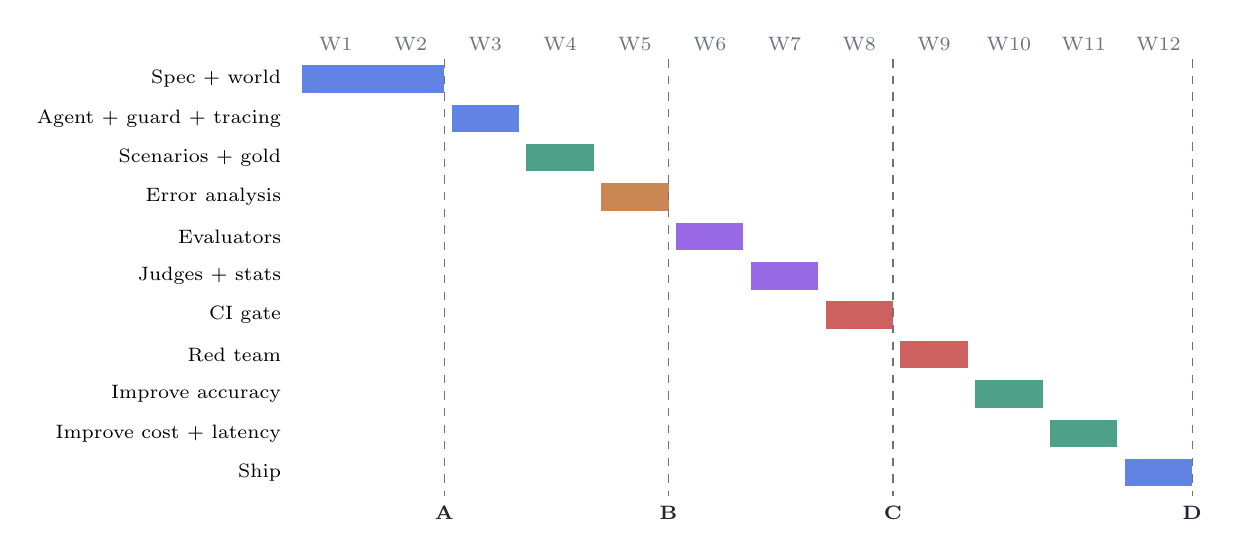
\begin{tikzpicture}[x=0.95cm,y=0.5cm]
  \foreach \w in {1,...,12} \node[font=\scriptsize,text=grey] at (\w+3.5,0.9) {W\w};
  \foreach \i/\name/\s/\e/\c in {
     0/Spec + world/1/2/accent, 1/Agent + guard + tracing/3/3/accent, 2/Scenarios + gold/4/4/good,
     3/Error analysis/5/5/warn, 4/Evaluators/6/6/purple1, 5/Judges + stats/7/7/purple1,
     6/CI gate/8/8/bad, 7/Red team/9/9/bad, 8/Improve accuracy/10/10/good,
     9/Improve cost + latency/11/11/good, 10/Ship/12/12/accent}{
    \node[anchor=east,font=\scriptsize] at (3.9,-\i) {\name};
    \fill[\c!70] (\s+3.05,-\i-0.35) rectangle (\e+3.95,-\i+0.35);
  }
  \foreach \w/\l in {2/A,5/B,8/C,12/D} \draw[dashed,grey] (\w+3.95,0.5) -- (\w+3.95,-10.6) node[below,font=\scriptsize\bfseries,text=ink]{\l};
\end{tikzpicture}
\end{center}

\begin{center}
\small
\begin{tabularx}{\linewidth}{@{}l l X@{}}
\toprule
\textbf{Checkpoint} & \textbf{Week} & \textbf{What exists}\\
\midrule
A & 2 & BazaarDW in both sizes, dictionary, metrics, planted facts tested\\
B & 5 & Agent with tracing, 930 eval items, failure taxonomy with counts\\
C & 8 & Validated judges, statistics, CI gate blocking regressions\\
D & 12 & Red-teamed, optimised, documented; headline results in the README\\
\bottomrule
\end{tabularx}
\end{center}

% =====================================================================
\section{Risks}

\begin{center}
\small
\begin{tabularx}{\linewidth}{@{}X X@{}}
\toprule
\textbf{Risk} & \textbf{Mitigation}\\
\midrule
Synthetic data too clean to be challenging & Built-in traps, dirty data and planted facts; check the error analysis shows varied failures; add traps if the agent passes too easily\\
Free tier cut, model retired or quota hit & Multi-provider fallback, local Ollama config, disk cache, resumable runs, \code{make models-check} before each phase\\
Gold SQL contains mistakes & Double-written check on the full size; planted-fact assertions; review every gold query by hand\\
Judges disagree with labels & More labelled examples; tighter rubrics; replace judge with a code check where possible\\
Overfitting to the eval set & Frozen test split; refresh dev items from new traces\\
Tool and model versions change & Versions in config and lock files; upgrade drill re-runs everything\\
Scope creep & Non-goals above; stretch items only after week 12 criteria pass\\
\bottomrule
\end{tabularx}
\end{center}

% =====================================================================
\section{Glossary}

\begin{center}
\small
\begin{tabularx}{\linewidth}{@{}l X@{}}
\toprule
Execution accuracy & Share of items where the agent's result rows equal the gold result rows\\
Gold SQL & A hand-verified query whose result is the correct answer\\
Size (small / full) & The two builds of BazaarDW: about 1 lakh and about 10 lakh rows\\
SCD2 & Slowly changing dimension type 2: history rows with \code{valid\_from} and \code{valid\_to}\\
Semantic layer & One file of official metric definitions shared by the agent and the evals\\
Schema retrieval recall & Share of the needed tables that the schema search returned\\
pass\^{}k & Probability that all $k$ repeated runs succeed (reliability)\\
TPR / TNR & Share of real failures / real passes that a judge labels correctly\\
Trace & The full record of one agent run: model calls, tool calls, guard decisions, cost\\
\bottomrule
\end{tabularx}
\end{center}

% =====================================================================
\clearpage
\appendix
\section{Appendix: Full Column List}

\textcolor{bad}{Red}: personal data. \textcolor{warn}{Orange}: untrusted free text. Primary key
is the first column (except \code{inventory\_snapshots}, keyed on snapshot date, warehouse and variant).

{\small
\begin{longtable}{@{}l l >{\raggedright\arraybackslash}p{9.3cm}@{}}
\toprule
\textbf{Table} & \textbf{Domain} & \textbf{Columns}\\
\midrule
\endfirsthead
\toprule
\textbf{Table} & \textbf{Domain} & \textbf{Columns}\\
\midrule
\endhead
\code{regions} & Reference & \footnotesize\ttfamily region\_id, name, name\_bn, population\_m\\
\code{cities} & Reference & \footnotesize\ttfamily city\_id, region\_id, name, name\_bn, is\_metro, courier\_zone\\
\code{calendar\_dim} & Reference & \footnotesize\ttfamily date\_key, date, year, quarter, month, month\_name, week\_of\_year, day\_of\_week, is\_weekend, is\_holiday, holiday\_name, fiscal\_year\\
\code{currency\_rates} & Reference & \footnotesize\ttfamily rate\_date, currency, bdt\_per\_unit, source\\
\code{customers} & Customers & \footnotesize\ttfamily customer\_id, \textcolor{bad}{full\_name}, \textcolor{bad}{email}, \textcolor{bad}{phone}, gender, birth\_year, city\_id, signup\_at, signup\_channel, acquisition\_source, is\_verified, preferred\_language, is\_deleted, updated\_at\\
\code{customer\_addresses} & Customers & \footnotesize\ttfamily address\_id, customer\_id, city\_id, \textcolor{bad}{street\_address}, \textcolor{bad}{postcode}, address\_type, is\_default, created\_at, is\_deleted\\
\code{customer\_segment\_history} & Customers & \footnotesize\ttfamily segment\_hist\_id, customer\_id, segment, valid\_from, valid\_to, is\_current\\
\code{loyalty\_accounts} & Customers & \footnotesize\ttfamily loyalty\_id, customer\_id, tier, points\_balance, enrolled\_at, status\\
\code{loyalty\_transactions} & Customers & \footnotesize\ttfamily loyalty\_txn\_id, loyalty\_id, order\_id, txn\_type, points, txn\_at, expires\_at\\
\code{categories} & Catalog & \footnotesize\ttfamily category\_id, parent\_category\_id, name, level, path\\
\code{brands} & Catalog & \footnotesize\ttfamily brand\_id, name, country, is\_local\\
\code{products} & Catalog & \footnotesize\ttfamily product\_id, seller\_id, brand\_id, category\_id, name, description, list\_price\_bdt, created\_at, status, is\_deleted, weight\_g, is\_imported\\
\code{product\_variants} & Catalog & \footnotesize\ttfamily variant\_id, product\_id, sku, size, colour, price\_delta\_bdt, barcode, is\_active\\
\code{product\_price\_history} & Catalog & \footnotesize\ttfamily price\_hist\_id, variant\_id, price\_bdt, valid\_from, valid\_to, change\_reason\\
\code{sellers} & Sellers & \footnotesize\ttfamily seller\_id, name, legal\_name, city\_id, joined\_at, seller\_type, \textcolor{bad}{contact\_email}, \textcolor{bad}{contact\_phone}, status, rating\_avg\\
\code{seller\_tier\_history} & Sellers & \footnotesize\ttfamily tier\_hist\_id, seller\_id, tier, valid\_from, valid\_to\\
\code{seller\_payouts} & Sellers & \footnotesize\ttfamily payout\_id, seller\_id, period\_start, period\_end, gross\_bdt, commission\_bdt, paid\_at\\
\code{warehouses} & Inventory & \footnotesize\ttfamily warehouse\_id, name, city\_id, capacity\_units, opened\_at, is\_active\\
\code{inventory\_snapshots} & Inventory & \footnotesize\ttfamily snapshot\_date, warehouse\_id, variant\_id, on\_hand\_units, reserved\_units, reorder\_point\\
\code{orders} & Orders & \footnotesize\ttfamily order\_id, customer\_id, address\_id, order\_at, status, channel, currency, total\_amount, total\_bdt, promo\_id, is\_deleted, updated\_at, device\_type\\
\code{order\_items} & Orders & \footnotesize\ttfamily order\_item\_id, order\_id, variant\_id, seller\_id, quantity, unit\_price, discount\_bdt, line\_total\_bdt, is\_gift\\
\code{order\_status\_events} & Orders & \footnotesize\ttfamily event\_id, order\_id, status, event\_at\_utc, actor\\
\code{payments} & Payments & \footnotesize\ttfamily payment\_id, order\_id, method, provider, attempt\_no, status, amount\_bdt, created\_at\_utc, captured\_at\_utc\\
\code{refunds} & Payments & \footnotesize\ttfamily refund\_id, order\_id, payment\_id, amount\_bdt, reason, requested\_at, processed\_at\\
\code{returns} & Payments & \footnotesize\ttfamily return\_id, order\_item\_id, quantity, reason, status, requested\_at, received\_at, refund\_id\\
\code{couriers} & Logistics & \footnotesize\ttfamily courier\_id, name, service\_level, is\_third\_party\\
\code{shipments} & Logistics & \footnotesize\ttfamily shipment\_id, order\_id, courier\_id, warehouse\_id, shipped\_at\_utc, promised\_date, delivered\_at\_utc, status, shipping\_fee\_bdt, attempt\_count\\
\code{shipment\_events} & Logistics & \footnotesize\ttfamily shipment\_event\_id, shipment\_id, event\_type, event\_at\_utc, city\_id, \textcolor{warn}{note}\\
\code{marketing\_campaigns} & Marketing & \footnotesize\ttfamily campaign\_id, name, channel, start\_date, end\_date, budget\_bdt, objective, owner\_team\\
\code{promotions} & Marketing & \footnotesize\ttfamily promo\_id, campaign\_id, code, promo\_type, discount\_value, min\_order\_bdt, start\_at, end\_at, max\_redemptions\\
\code{promotion\_redemptions} & Marketing & \footnotesize\ttfamily redemption\_id, promo\_id, order\_id, customer\_id, discount\_bdt, redeemed\_at\\
\code{web\_sessions} & Web & \footnotesize\ttfamily session\_id, customer\_id, started\_at\_utc, ended\_at\_utc, device\_type, traffic\_source, campaign\_id, landing\_page, pages\_viewed, added\_to\_cart, converted\_order\_id\\
\code{support\_tickets} & Support & \footnotesize\ttfamily ticket\_id, customer\_id, order\_id, channel, category, priority, status, created\_at\_utc, resolved\_at\_utc, agent\_id\\
\code{support\_messages} & Support & \footnotesize\ttfamily message\_id, ticket\_id, sender\_type, sent\_at\_utc, \textcolor{warn}{body}, language\\
\code{product\_reviews} & Reviews & \footnotesize\ttfamily review\_id, product\_id, customer\_id, order\_id, rating, \textcolor{warn}{title}, \textcolor{warn}{body}, created\_at\\
\bottomrule
\end{longtable}
}

\end{document}
